\documentclass[12pt]{beamer}
\usetheme{Madrid}




\setbeamertemplate{footline}
{
  \leavevmode%
  \hbox{%

  \begin{beamercolorbox}[wd=.67\paperwidth,ht=2.25ex,dp=1ex,center]{title in head/foot}%
    \usebeamerfont{title in head/foot}\insertshorttitle
  \end{beamercolorbox}%
  \begin{beamercolorbox}[wd=.333333\paperwidth,ht=2.25ex,dp=1ex,right]{date in head/foot}%
    \usebeamerfont{date in head/foot}\insertshortdate{}\hspace*{2em}
    \insertframenumber{} / \inserttotalframenumber\hspace*{2ex} 
  \end{beamercolorbox}}%
  \vskip0pt%
}

\usepackage[T1]{fontenc}
\usepackage[utf8x]{inputenc}
\usepackage[francais]{babel}

\usepackage{graphicx}
\usepackage{lmodern}
\author{ALIJATE Mehdi -  NEGROS Hadrien- TURKI Batoul}
\title{TER :  Intégration et optimisation d’algorithmes de classifications supervisées pour Weka
}
%\setbeamercovered{transparent} 
%\setbeamertemplate{navigation symbols}{} 

\institute{Université Montpellier 2 - LIRMM} 
%\date{} 
%\subject{} 




<<<<<<< HEAD


=======
>>>>>>> 6837ff9d819b45eb2265beb68016fdd7f0f52829
\begin{document}



\begin{frame}
\titlepage 
\end{frame}

\AtBeginSection[]{
 \begin{frame}
    \frametitle{Sommaire}
    \tableofcontents[sectionstyle=show/shaded,subsectionstyle=hide/show/hide]
  \end{frame}

} 


\begin{frame}
\begin{abstract}

\frametitle{Abstract}
\begin{center}
Ce sujet vise à intégrer et à optimiser des algorithmes de classifications supervisées de documents dans la suite logiciel WEKA. Ces algorithmes sont issus de travaux de recherche menés récemment au sein du LIRMM.
\end{center}
\end{abstract}
\end{frame}

\begin{frame}
\tableofcontents
\frametitle{Sommaire}


\end{frame}


\section{Introduction}



\begin{frame}
\frametitle{Introduction}
\begin{block}{Introduction}
\begin{itemize}
\item Ce TER vise à intégrer des algorithmes de classifications supervisées de documents dans la suite logiciel WEKA 
\item Intégrant de nouvelles solutions adaptées aux faibles quantités de données textuelles.
\item Se basant sur de nouvelles pondérations.
\end{itemize} 
\end{block}
\end{frame}
\begin{frame}
\frametitle{La classification}
La classification est le processus visant à associer un document à la classe le représentant le mieux.
\begin{block}{Exemple}
Classer des résumés de films selon leur genre. (Policier, Comédie, etc...)
\end{block}
\begin{block}{Vocabulaire}
\begin{description}
\item[Attribut] Ou \textbf{terme unique} est un élément d'un document.
\item[Document] Un ensemble d'attributs (ex: un résumé)
\item[Classe] Un ensemble de documents liés entre eux. (ex: genre cinématographique)
\end{description}
\end{block}


\end{frame}

\begin{frame}
\frametitle{Besoins}
\begin{block}{Besoins}
\begin{itemize}
\item Prise en main de Weka
\item Développement des différentes bibliothèques en java
\item L'intégration dans l’écosystème Weka
\end{itemize}
\end{block}

\end{frame}

\section{Organisation}
\begin{frame}
\frametitle{Organisation}
\begin{itemize}
	\item Plusieurs réunions
	\item Un outil collaboratif pour la gestion du projet : Github
	\item Mises au point régulières
\end{itemize}
\end{frame}

\section{Exploration de WEKA}

\begin{frame}
\frametitle{Exploration de Weka}
\begin{itemize}
\item L'API Weka
\item L'utilisation des classes
\item Ajout d'un algorithme dans Weka
\end{itemize}
\begin{block}{A la fin de cette étape}
\begin{itemize}
\item Méthodes et classes ciblées
\item Le Package \textit{weka.classifiers}
\item Le classifieur \textit{NaiveBayesMultinomial}
\item Pour l'ajout d'algorithme : Le package \textit{weka.gui}
\end{itemize}
\end{block}
\end{frame}

\section{Nouvelles méthodes de classifications}

\begin{frame}
\frametitle{Nouvelles méthodes de classifications}
\begin{itemize}
\item Différentes pondérations pour la construction des nouveaux classifieurs
\begin{enumerate}
\item Des mesures intra-classe.
\item Des mesures inter-classe.
\end{enumerate}
\end{itemize}
Ces mesures sont inspirées du TF-IDF et ont étés développées au LIRMM.\\
Elles sont définies dans l'article:
\begin{center}
De nouvelles pondérations adaptées à la classification de petits volumes de données textuelles.\\
De \textit{M. Roche, F. Bouillot, P. Poncelet}\\
EGC 2014
\end{center}

\end{frame}

\begin{frame}
\frametitle{Pondérations intra-classe}
\begin{itemize}
\item Les pondérations que nous définissons ci-après sont dites \textbf{intra-classe} 
\item Les différentes valeurs que nous utilisons pour les calculer sont dépendantes d'une classe.
\end{itemize}
\end{frame}

\begin{frame}
\subsection{Pondérations intra-classe}
\frametitle{Intra-classe document}
\subsubsection*{intra-classe document}

Cette mesure dépend du nombre de documents contenant le terme dans la classe.
  \[ inner\mbox{-}weight_{ij}^{Df} = \frac{DF_{ti}^j}{|d_{j}|}\]
  
      Avec:
  \begin{itemize}
  	\item $DF_{ti}^j$: Nombre de documents contenant le terme $t_i$ dans la classe $C_j$	
  	\item $|d_{j}|$: Nombre de documents dans $C_j$	
    \end{itemize}
\end{frame}

\begin{frame}
\subsubsection*{intra-classe terme}
\frametitle{Intra-classe terme}
Cette mesure dépend du nombre d'occurrences du terme dans la classe.
\[   inner\mbox{-}weight_{ij}^{Tf} = \frac{TF_{ti}^j}{|n_{j}|}\]
  Avec:
\begin{itemize}
	\item $TF_{ti}^j$: Nombre d'occurrences du terme $t_i$ dans la classe $C_j$	
	\item $|n_{j}|$: Nombre de termes total dans la classe $C_j$	
  \end{itemize}
\end{frame}  





\begin{frame}
\frametitle{Pondérations inter-classe}
\begin{itemize}
\item Les pondérations inter-classes utilisent des valeurs calculées à partir de l'ensemble du corpus.

\item Depuis les classes extérieures à celle qui nous intéresse.
\end{itemize}
\end{frame}

\begin{frame}
\subsection{Pondérations inter-classe}
\frametitle{Inter-classe terme}
\subsubsection*{inter-classe terme}

Cette mesure dépend du nombre de classes contenant le terme.
\[inter\mbox{-}weight_{ij}^{class} = log_2 \frac{|C|}{C_{ti}}\]
Avec:
\begin{itemize}
	\item $|C|$: Nombre de classes			
	\item $C_{ti}$: Nombre de classes contenant le terme $t_i$
  \end{itemize}
\end{frame}
\subsubsection*{inter-classe document}

\begin{frame}
\subsubsection*{inter-classe document}
\frametitle{Formule inter-classe document}
Cette mesure dépend du nombre de documents extérieurs à la classe contenant le terme.
 \begin{small}
 

\[ inter\mbox{-}weight_{ij}^{doc} = log_2 \frac{|d \notin{C_j}|+1}{|d:t_i \notin{C_j}|+1}\]
 \end{small}
 Avec:
 \begin{small}
\begin{itemize}
	\item $|d \notin  {C_j}|$: Nombre de documents n'appartenant pas à la classe $C_j$
	\item $|d:t_i \notin {C_j}|$: Nombre de documents n'appartenant pas à la classe $C_j$ qui contient $t_i$ 
	\item En ajoutant 1, permet de prévenir le cas où $t_i$ est uniquement utilisé dans $C_j$ (quand $|d:t_i \notin{C_j}|={|d:t_i|-|d:t_i \in{C_j}|} = 0$)
  \end{itemize}
 \end{small}
\end{frame}  
\subsection{Algorithmes de classifications}
\begin{frame}
\frametitle{Algorithmes de classifications}

\begin{itemize}
\item Nous avons implémenté un classifieur \textit{Naive Bayes} et \textit{Class-Feature-Centroid}. 
\item Pour calculer la probabilité $w_{ij}$ d'un terme $i$ dans une classe $j$, nous avons combiné les différentes pondérations de 4 façons:
\end{itemize}

\end{frame}
\begin{frame}
\frametitle{Les quatres pondérations}

\begin{itemize}
\item $w_{ij}^{Tf-Class}$=$inner$-$weight_{ij}^{Tf}$ $\times$ $inter$-$weight_{ij}^{class}$
%=$ \frac{TF_{ti}^j}{|n_{j}|}$ x $log_2 \frac{|C|}{CF_{ti}}$
\item $w_{ij}^{Df-Class}$=$inner$-$weight_{ij}^{Df}$ $\times$ $inter$-$weight_{ij}^{class}$
%=$\frac{DF_{ti}^j}{|d_{j}|}$ x $log_2 \frac{|C|}{CF_{ti}}$
\item $w_{ij}^{Tf-Doc}$=$inner$-$weight_{ij}^{Tf}$ $\times$ $inter$-$weight_{ij}^{doc}$
%=$ \frac{TF_{ti}^j}{|n_{j}|}$ x $log_2 \frac{|d|-|d \in{C_j}|+1}{|d:t_i|-|d:t_i \in{C_j}|+1}$
\item $w_{ij}^{Df-Doc}$=$inner$-$weight_{ij}^{Df}$ $\times$ $inter$-$weight_{ij}^{doc}$
%=$\frac{DF_{ti}^j}{|d_{j}|}$ x $log_2 \frac{|d|-|d \in{C_j}|+1}{|d:t_i|-|d:t_i \in{C_j}|+1}$
\end{itemize}
\begin{block}{Paramètres : $\alpha,\beta$}


Nous avons aussi mis en place une combinaison de ces mesures dépendantes de deux paramètres $\alpha,\beta \in [0,1]$:
\begin{center}
 $w_{ij}^{ \alpha \beta}=(\alpha \times inner$-$weight_{ij}^{Tf} + (1-\alpha)\times inner$-$weight_{ij}^{Df} )\times(\beta \times inter$-$weight_{ij}^{class} + (1-\beta) \times inter$-$weight_{ij}^{doc} )$
\end{center}
\end{block}
\end{frame}


\section{Développement des algorithmes de classifications}
\begin{frame}
\frametitle{Développement}

\begin{description}
\item[buildClassifier()]  C'est la méthode dans laquelle est calculé le tableau des $w_{ij}$ (La probabilité d'un mot par rapport à une classe).
\item[distributionForInstance(Instance)] Renvoie les probabilités du document (Instance) en entrée pour chacune des classes du corpus.
\end{description}


\end{frame}



\subsection{NBMultinomialTER}
\begin{frame}
\frametitle{NaiveBayesMultinomialTER}

\begin{description}
\item[Version 1 : ]  implémentant les quatre pondérations.
\item[Version 2 : ] paramètrable avec $\alpha$ et $\beta$
\end{description}


\end{frame}

\begin{frame}
\frametitle{CFCTERab}
\subsection{CFCTERab}
\begin{itemize}
\item Représentation des classes comme des vecteurs (exemple: $\vec{C_j} = (0.1,0.3,0.2,0)$)
\item Représentation des documents comme des vecteurs (exemple: $\vec{d} = (0.1,0,0.2,0)$, le terme 2 n'apparait pas dans le document)
\item Mesure de la proximité entre les vecteurs en utilisant la proximité cosinus :
\[simcos(\vec{u},\vec{v}) = arccos( \frac{\vec{u}.\vec{v}}{\|\vec{u}\|.\|\vec{v}\|})\]
\end{itemize}



\end{frame}





\section{Intégration et résultats}
\subsection{Intégration}
\begin{frame}
\frametitle{Intégration}

\begin{center}
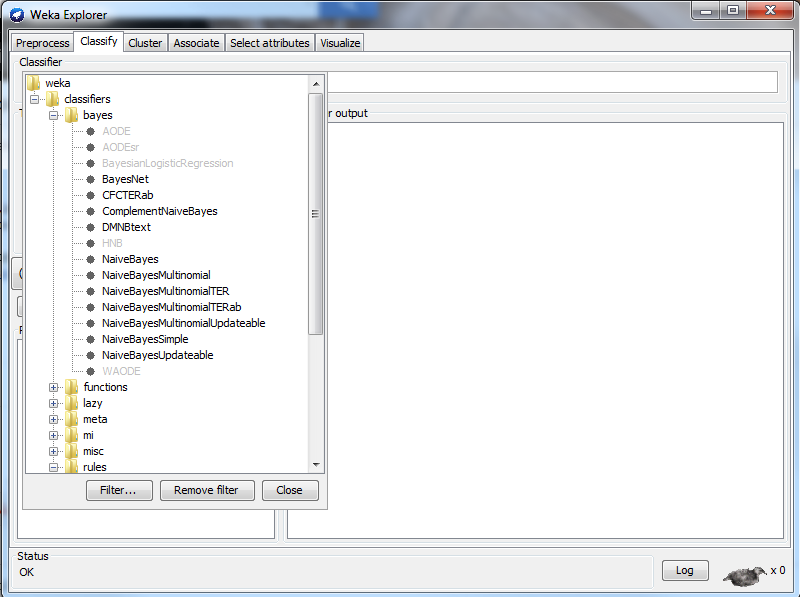
\includegraphics[width=0.80\textwidth]{wekaAlgos}~\\[1cm]  
\end{center}


\end{frame}


\begin{frame}
\frametitle{Tests}
Classification de résumés de films.
\begin{center}
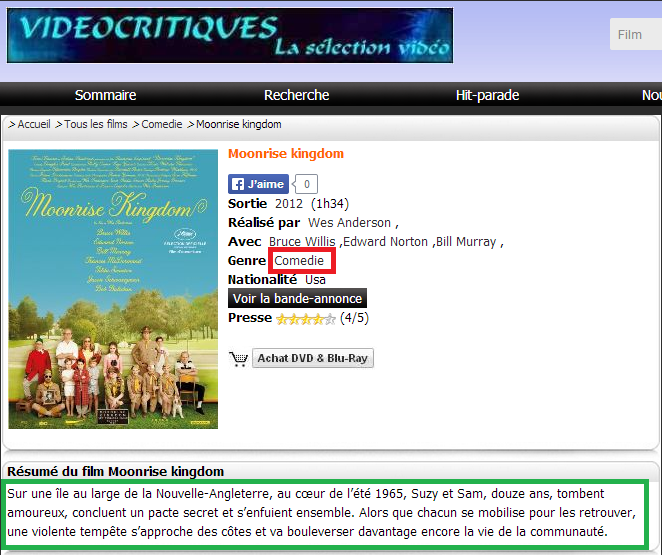
\includegraphics[width=0.70\textwidth]{vc}
\end{center}

\end{frame}

\begin{frame}
\frametitle{Jeux de données}

Nos jeux de données : 
\begin{itemize}
\item \texttt{\textbf{test3classes.arff}} : \textbf{150} instances et \textbf{41} attributs (une selection d'attributs \textbf{SubsetEval} a été faite dessus), avec \textbf{3} classes : Policier, Fantastique, Comédie.
\item \texttt{\textbf{test5classes.arff}} : \textbf{248} instances et \textbf{5082} attributs au complet (sans selection d'attributs), avec \textbf{5} classes : Thriller, Western, Guerre, Policier, Sciences.
\end{itemize}


\end{frame}




\subsection{Résultats des tests}
\begin{frame}
\frametitle{Résultats des tests : NaiveBayesMultinomialTER}


\begin{table}
\centering
    \begin{tabular}{|l|c||c|}
    \hline
    NBMultinomialTER/fichierTest  & $Nb^{Df-Class}$ & NBMultinomial \\ \hline
    test3classes.arff & \textbf{67\%}   & 66\%  \\ \hline
    test5classes.arff & \textbf{68\%} & 63\%  \\ \hline
    \end{tabular}
\end{table}
\medskip
Expérimentations avec $Nb^{Df-Class}$ et comparaison avec NBMultinomial
\end{frame}

\begin{frame}
\frametitle{Résultats des tests : NBTER $\alpha\beta$ et CFCTER$\alpha\beta$ }
\begin{footnotesize}



\begin{table}


    \begin{tabular}{|l|c|c|c|c||c|}
\hline
 Algo/FichierTest & $\alpha$ & $\beta$ & NBMTER$\alpha\beta$ & CFCTER$\alpha\beta$ & NBMulti \\
    \hline
    test3classes.arff &  0.0 &  1.0& \textbf{67\%} & 68\% & 66\% \\
    \cline{2-5}
         ~ &   0.6  &  0.6 & 66\% & \textbf{74\%} & ~\\
         \cline{2-5}
         ~ &   0.7  &  0.3 & 66\% & 73\% & ~\\
    \hline
     test5classes.arff &  0.0 &  1.0& \textbf{67\%} &68\% & 63\% \\
    \cline{2-5}
         ~ &   0.6  &  0.6 & 65\% & \textbf{70\%} & ~\\
         \cline{2-5}
         ~ &   0.7  &  0.3 & 58\% & 60\% & ~\\
    \hline
    \end{tabular}
\end{table}
\end{footnotesize}
\medskip
Expérimentations avec différentes valeurs de $\alpha$  \ et $\beta$ \  pour NBTER$\alpha\beta$ \ et CFCTER$\alpha\beta$ 
\end{frame}



\section{Conclusion}
\begin{frame}
\frametitle{Conclusion}
Ce TER nous a permis de :
\begin{itemize}
\item Prendre en main  Weka 
\item Comprendre les nouvelles mesures de classification
\item Intégrer les algorithmes dans l’écosystème Weka 
\end{itemize}
\begin{block}{Perspective}
Implémenter de nouvelles métriques pour CFC (exemple : Distance de Jaccard)
\end{block}

\end{frame}
\begin{frame}

\begin{center}
\huge Démonstration

\end{center}
\end{frame}
\section{Démonstration}



\end{document}